
\section{Implementation of a prototypical micro-frontend architecture}

The first step was to implement a prototypical micro-frontend architecture that fits my companies needs. Runtime integration was chosen to take the most advantages of micro front-ends. To implement the runtime

The micro-frontend architecture that powers the prototype was developed using Webpack's Module Federation. The prototype contains a shell-application that loads all other micro-frontends. The architecture is divided into 9 widgets that display only simple data and 3 complex single-page applications.

The main part of the implementation is written in Angular. One micro-frontend was implemented with the frontend-framework React to show that the findings of this project are technology agnostic.

I implemented one micro-frontend in React to show that the architecture is technology agnostic and if it can access the shared Apollo caching layer. For loading and rendering the React micro-frontend inside the host, I had to implement an adapter inside the shell-application. This adapter renders the React application inside a HTMLElement. It also provides the necessary configuration like the instance of the Apollo cache as context to the application.

Every micro-frontend is a complete Angular application that offers all of the features that Angular offers.

A rough overview of the architecture is shown in figure \ref{figure:methods:ui-dashboard-architecture}. The icons inside the squares represent the technology used.

\ifshowImages
\begin{figure}[H]
\centering
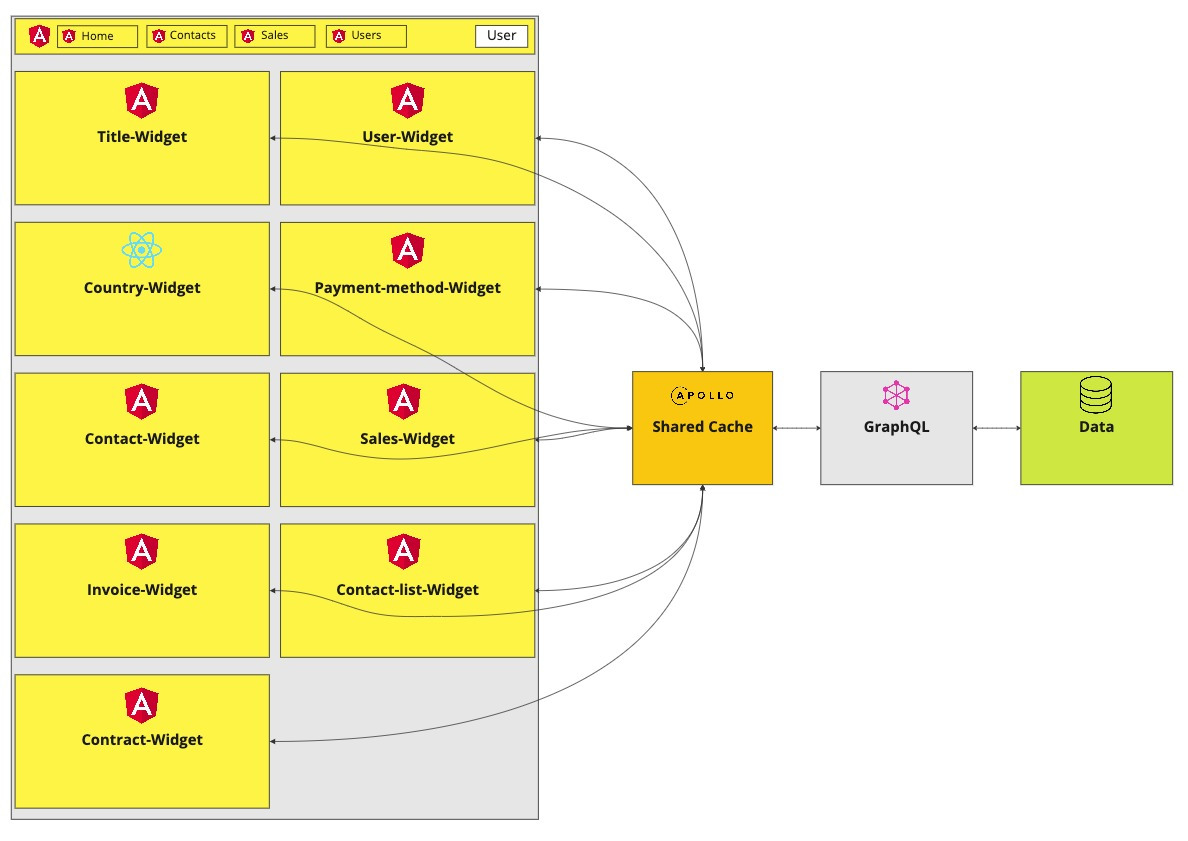
\includegraphics[width=0.8\linewidth]{images/ui-dashboard-architecture.jpeg}
\caption{Architecture of the micro-frontend prototype.}\label{figure:methods:ui-dashboard-architecture}
\end{figure}
\fi

The functionality of the micro-frontends is encapsulated in modules that can be used by the shell application. Each icon of Angular and React represents such a module, as shown in figure \ref{figure:methods:ui-dashboard-architecture}. These modules can be used when the application is running in standalone mode, and the modules can be made accessible to the shell application via module federation.

How a module can be exposed to be consumed by a remote application is shown in the listing \ref{code:methods:module-federation-config-expose}.

\ifshowListings
\begin{listing}[H]
\begin{minted}{typescript}
module.exports = {
  name: 'contact',
  exposes: {
    './Module': 'apps/contact/src/app/remote-entry/entry.module.ts',
  },
};
\end{minted}
\caption{Module Federation config to expose an Angular module to be consumed.}\label{code:methods:module-federation-config-expose}
\end{listing}
\fi

The host can configure its Module Federation to to be able to consume the entry.module.ts from the contact micro-frontend. The configuration can be seen in the listing \ref{code:methods:module-federation-config-consume}.

\ifshowListings
\begin{listing}[H]
\begin{minted}{typescript}
module.exports = {
  name: 'host',
  remotes: {
    contact: 'contact@http://localhost:4202/remoteEntry.js'
  },
};
\end{minted}
\caption{Module Federation config that consumes an Angular module from a remote location.}\label{code:methods:module-federation-config-consume}
\end{listing}
\fi

Inside the host application the remote module from the contact application can be easily referenced and routed to. The configuration of the route can be seen in listing \ref{code:methods:angular-route-to-remote-module}

\ifshowListings
\begin{listing}[H]
\begin{minted}{typescript}
const routes: Routes = [
  {
    path: 'contact',
    loadChildren: () =>
    loadRemoteModule(
      'contact',
      './Module'
    ).then((m) => m.UiContactRemoteEntryModule),
  },
  ...
]
\end{minted}
\caption{Route to the exposed remote-module from the contact application}\label{code:methods:angular-route-to-remote-module}
\end{listing}
\fi


\subsection{Module Federation}

\subsection{Integrating react micro-frontend}

\subsection{Backend for frontend architecture}